\section{Quote manager scaling}
The system's TPS grows almost $10\times$ once a full set of quotes has been retrieved. further increases to average TPS could be gained by decreasing the time spent fetching quotes.
The methods in~\ref{sec:qs} brought the quote server response time to its lower limit so further efficiency could only come from horizontally scaling the quote managers.
Intuitively, doubling the number of quote managers should decrease the total time to retrieve all quotes by half, provided the workload is split evenly.
If only it were so simple.

\subsection{Building a ``snoopy'' quote manager}
With one week until the final deadline we decided to refactor the quote manager to participate in a multi-quote manager environment.
We ported the ``snoopy caching'' functionality from the worker and audit logger into the quote manager.
The ``snoopy'' quote server could listen to quote broadcasts and update its local cache accordingly.
With this functionality, multiple quote managers could act as workers servicing requests from a single RMQ queue. 

A message header with the ID of the quote manager that serviced the request was added to all quote broadcasts.
The quote manager cache updaters would discard messages that originated from its own quote manager.
This is inefficient but necessary because RMQ does not allow an ``anti-match'' for message routing keys.
That is, one cannot specify, "Capture all messages \textit{except} ones that follow this pattern.''

Total development effort was approximately one hour.

\subsection{Performance analysis}
Figure~\ref{fig:snoopy-qs} shows that TPS correlates \textit{negatively} with the number of snoopy quote managers.
This is very counter-intuitive and deserves reflection.

\begin{figure}[tbph]
  \centering
  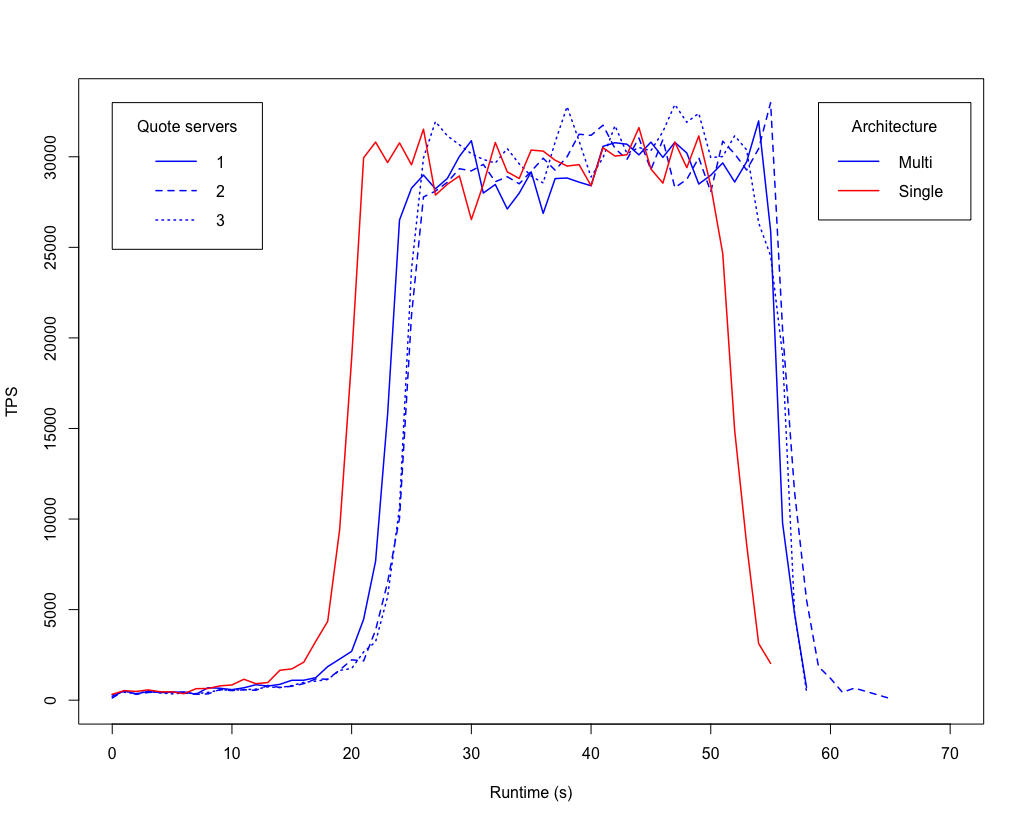
\includegraphics[width=0.85\linewidth]{../../data/tps/multi_vs_single_qs}
  \caption[Snoopy quote manager performance]{Performance of multi and single quote manager designs on 1000 user workload}
  \label{fig:snoopy-qs}
\end{figure}

Comparing the single quote manager deployment in multi and single architectures gives a sense of the overhead associated with discarding quote broadcasts.
The relation becomes less clear when two and three quote managers are used: the system benefits from having to retrieve fewer quotes per quote manager but adding quotes to the cache also has a delay.
The benefits from horizontal scaling start to manifest when three quote managers are used, but it takes the form of, ``things stopped getting worse,'' instead of ``performed better than a single quote manager.''

The single architecture quote manager is very fast because it already functions like a multi machine quote manager.
Each new request spawns a thread that handles communication with the legacy service.
Most of the threads are blocking on a response from the legacy service making it very likely that a new thread will find the application in an idle state.
Since workers block on the completion of a quote command the maximum number of simultaneous quote requests is equal to the number of workers.
Hence, the number of threads requesting quotes in the quote manager is capped, thus preventing thread creation runaways and CPU starvation in the quote manager.
Adding more quote managers doesn't increase the number of simultaneous quotes that can be requested by workers.

\subsection{Alternate solutions}
The snoopy quote manager was implemented because it was a small amount of development effort for a large potential payoff.
There is another way to implement multiple quote managers, although it is more complicated: quote symbols could be hashed to associate with unique quote managers.
This prevents the need for quote managers to do snoopy caching.
However, it introduces problems with scaling since the hash will depend on the number of available quote managers.

The snoopy quote manager can scale easier since failures would be independent.
As the number of workers continues to grow, Figure~\ref{fig:snoopy-qs} should be re-run to determine the break point between the communication overhead and the increased capacity for simultaneous quote requests.

